\section{Architecture}
\label{chap:proposal:architecture}

\begin{figure}[tp]
    \centering
    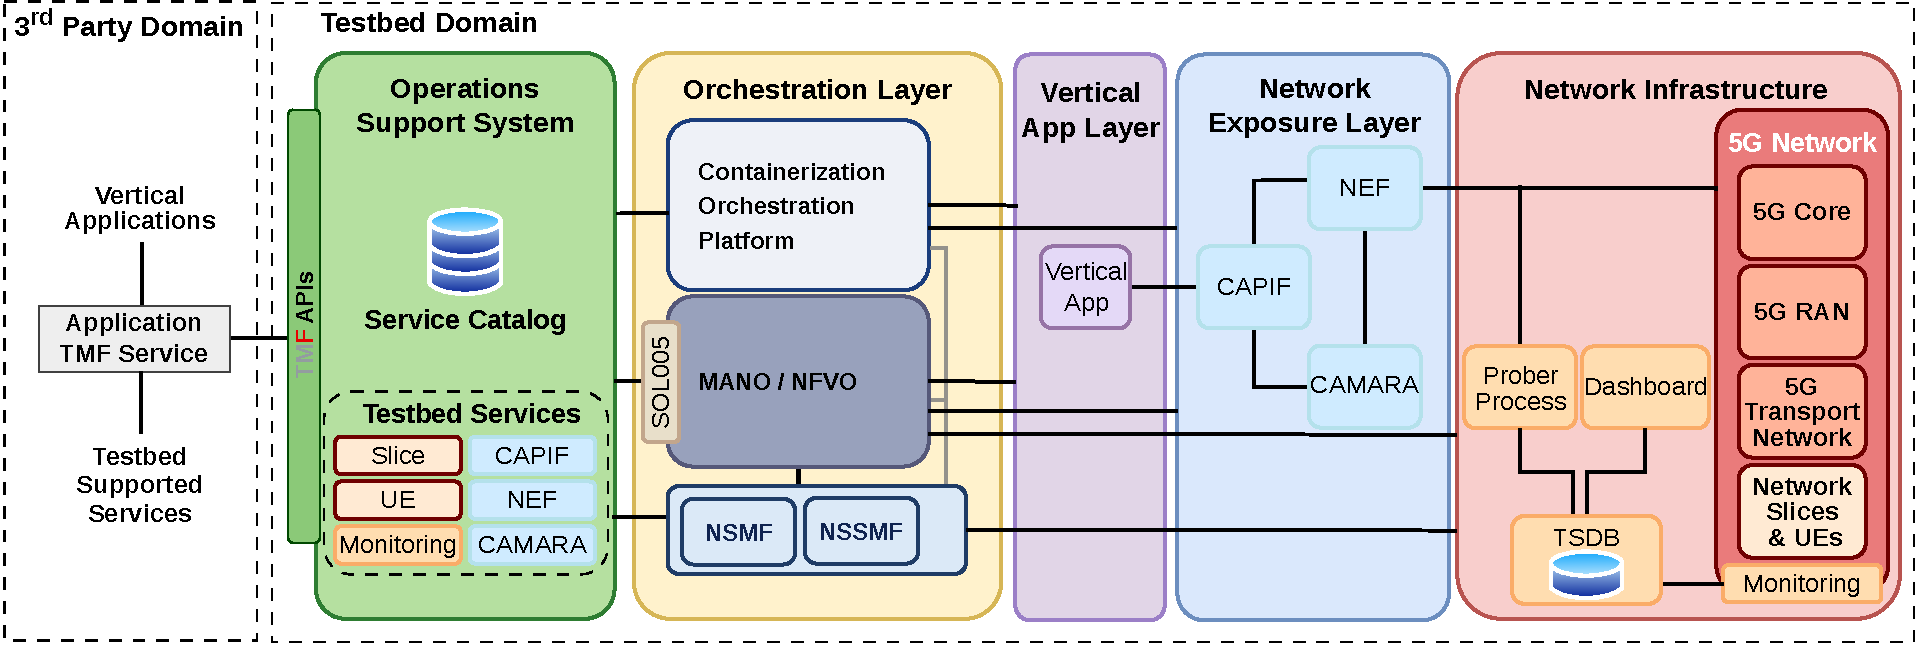
\includegraphics[width=1\linewidth]{figs/drawio/proposed_architecture.pdf}
    \caption{Proposed Testbed Architecture}
    \label{fig:proposal:architecture}
\end{figure}

According to the objectives delineated in Section \ref{chap:introduction:objectives}, the proposed testbed should offer vertical industries an experimentation environment to develop and validate network applications over a real \acs{5G} system. Figure~\ref{fig:proposal:architecture} shows the proposed architecture, separating the third-party domain, where verticals order and manage their experiments, from the testbed domain, where experiments are deployed and executed. The testbed domain follows a layered structure comprising an Operations Support System, the orchestration layer, the vertical application layer, the network exposure layer and the network infrastructure, including network monitoring.

For this purpose, third parties must be able to self-provision complete network environments tailored to their application requirements, without needing to interact with the underlying infrastructure. To this end, the \acs{OSS} should act as the main entry point to the testbed for all interactions regarding the ordering and provisioning of resources. Complete experiments comprise interdependent components, including slices, \acsp{UE}, exposure interfaces, monitoring, and vertical applications, which may rely on distinct deployment mechanisms, often through proprietary interfaces. Requiring verticals to interact with these components directly would expose internal details of the testbed, demand technology-specific knowledge, and introduce manual configuration, compromising reproducibility.

Instead, the \acs{OSS} should expose \acs{TMF} Open \acsp{API} following the \acs{TMF} \acs{ODA}, allowing verticals to discover, order, and manage services through standardized interfaces, independently of how they are realized. Centralizing experiment provisioning through the \acs{OSS} would ensure each experiment is instantiated consistently, in the order imposed by their dependencies. The services offered by the testbed should be published in a service catalog within the \acs{OSS}. Vertical applications should also be onboarded into this catalog as \acs{TMF} services, as the other testbed services. Their design and delivery workflows are detailed in Section~\ref{chap:proposal:delivery}.

Nevertheless, an \acs{OSS} is not an orchestrator and should delegate the orchestration and provisioning of resources and network applications to the orchestration layer, which would host the components responsible for the actual deployment and lifecycle management of each resource. As the testbed must accommodate both cloud-native and virtualized workloads, this layer should include a container orchestration platform and a \acs{NFVO}, integrated via the \acs{ETSI} \acs{SOL}005 interface. The former would deploy containerized components, such as the vertical applications, the exposure components and the monitoring components, while the latter would deploy \acs{NFV}-based network services.

To accommodate the diverse \acs{QoS} requirements of applications across different vertical sectors, and enable multiple experiments to coexist on a shared physical infrastructure, network slicing should be employed, establishing isolated logical networks tailored to the specific needs of each experiment. For this reason, orchestration layer must also include the \acs{NSMF} and the \acs{NSSMF}, to which the \acs{OSS} forwards the network slice requirements derived from each slice. The \acs{NSMF} manages the lifecycle of each \acs{NSI} and delegates its constituent \acsp{NSSI} to the \acs{NSSMF}, which configures the corresponding resources across the \acs{5G} network, relying on the \acs{NFVO} whenever virtualized network functions must be orchestrated.

The vertical application layer should host the network applications developed by third parties, deployed by the orchestration layer once ordered through the \acs{OSS}. Although these applications would run within the testbed domain, their only means of interacting with the \acs{5G} network should be the network exposure layer, through which they could adapt the network to their requirements and react to changes in network conditions. This leads to another key objective of this dissertation: the secure exposure of network capabilities via northbound \acsp{API}.

As highlighted in Section~\ref{sec:sba:nef}, the \acs{NEF} is the core network function of the \acs{5G} \acs{SBA} responsible for securely exposing network capabilities and events to third parties. The testbed follows this same principle, relying on the \acs{NEF} as the main gateway for \acs{5G} programmability. However, leveraging these capabilities typically requires an understanding of the underlying \acs{3GPP} procedures, which introduces a significant barrier for vertical developers who may lack the specialized telecom expertise.

To address this challenge, CAMARA services should be introduced, providing a standardized set of network \acsp{API} that act as a translation layer between the complex \acs{3GPP} \acs{NEF} and developer-friendly interfaces, at the cost of reduced control over the network. Offering both interfaces would allow each vertical to select the abstraction level that best fits its application and expertise level. As the exposure interfaces are offered to external parties, there is also a need of a common governance mechanism for the secure publication, discovery and consumption of all testbed northbound \acsp{API}, which should be fulfilled by \acs{CAPIF}.

Lastly, the network infrastructure layer should encompass the \acs{5G} system over which experiments are executed, comprising the \acs{5GC}, the \acs{RAN} and the \acs{TN}. To support adaptive application behavior, the testbed must monitor the network autonomously. This requires monitoring components to be integrated with the network infrastructure, storing the collected metrics on a \ac{TSDB}, through which they can be made available to third parties via the testbed's exposure \acsp{API}, i.e. \acs{NEF} and CAMARA. The testbed should support both passive (autonomous) and active (probing) monitoring approaches, which should both be observable by the experimenter through visual dashboards. In order to validate the testbed, a \acs{5G} network application will be onboardded and developed leveraging the envisioned northbound interfaces, catering to the specific requirements of the \acs{PPDR} and automotive vertical sectors.
